\documentclass{beamer}
\usepackage{graphicx}
\usepackage[spanish]{babel}
\usepackage[utf8]{inputenc}
\setbeamertemplate{navigation symbols}{}
\usepackage{beamerthemeshadow}
\begin{document}
\title{Aplicaciones Web Desconectadas}
\author{Defossé Nahuel, van Haaster Diego Marcos}
\date{15 de Diciembre de 2009}

\begin{frame}
\titlepage
\end{frame}

\section{Introducción}
\subsection{Contexto}

\begin{frame}
    \frametitle{¿Qué es Web?}
    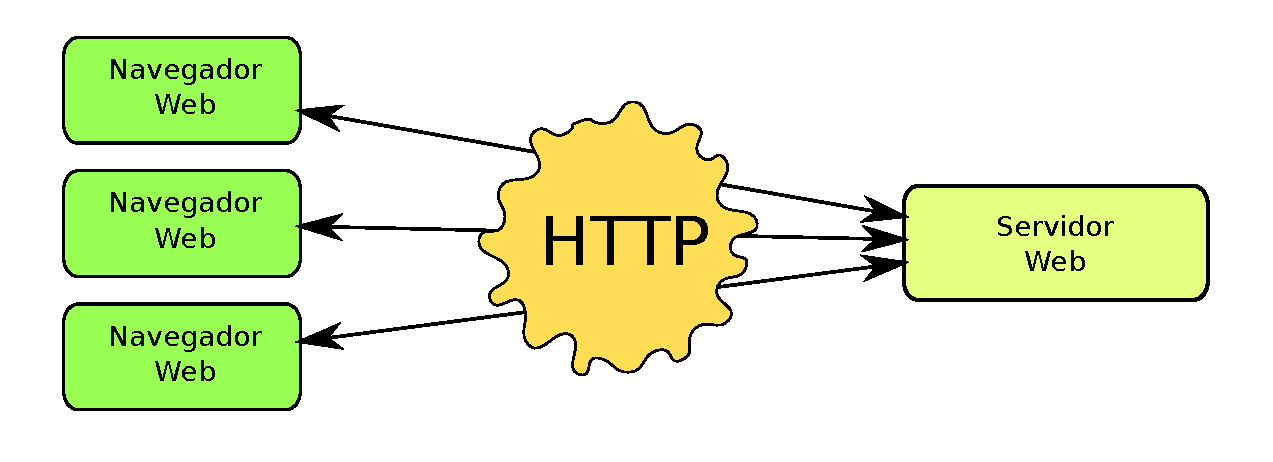
\includegraphics[scale=0.5]{intro.pdf}
\end{frame}
    

\begin{frame}
    \frametitle{¿Qué es una aplicación Web?}
    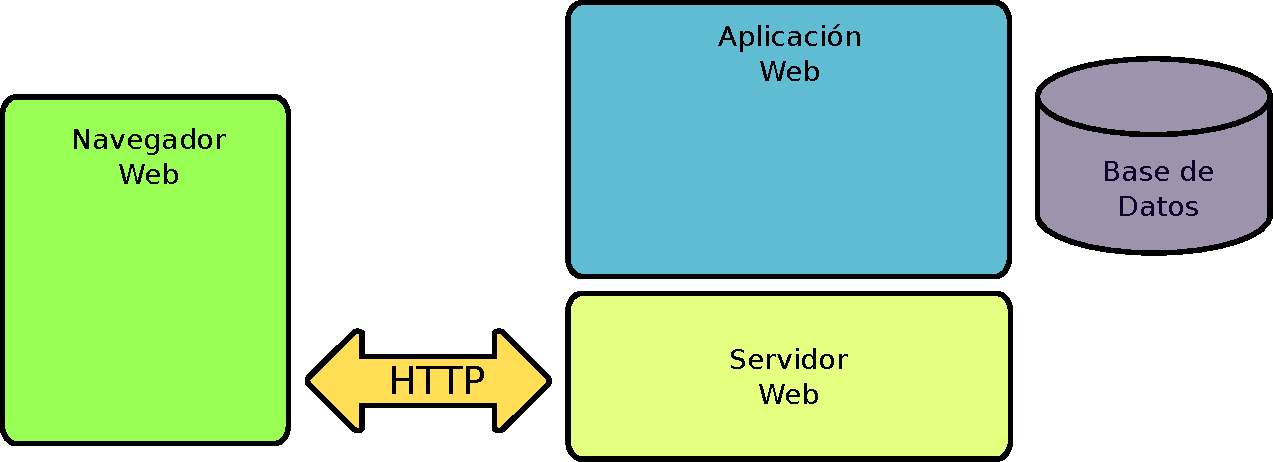
\includegraphics[scale=0.5]{general.pdf}
\end{frame}

\begin{frame}
    \frametitle{¿Qué es una aplicación Web Hoy?}
    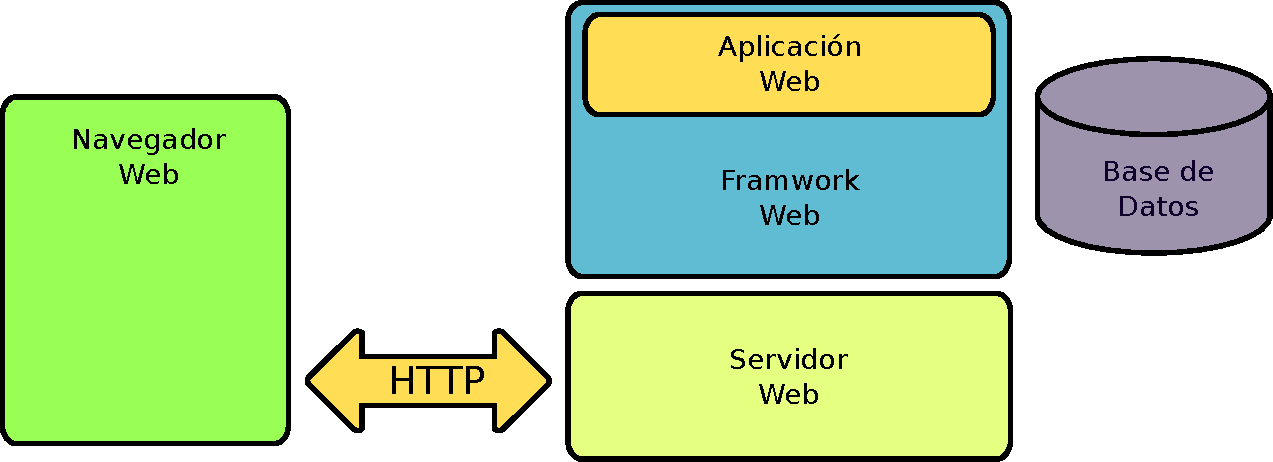
\includegraphics[scale=0.5]{general_con_fw.pdf}
\end{frame}

\subsection{Objetivos}
\begin{frame}
    \frametitle{Objetivos}
    \begin{block}{Objetivo Principal}
    
    ``Extender un framework de aplicaciones web existente, {\bf Open Source},
              de manera que una aplicación realizada sobre éste pueda ser ejecutada
              en el cliente de manera desconectada con un mínimo de modificaciones.
              Para permitir que la aplicación pueda ejecutarse en el cliente, se
              implementará:''
        \begin{itemize}
        \item Persistencia del modelo de datos en el cliente
        \item Subconjunto de acciones disponibles en modo desconectado
        \item Primitivas de sincronización entre la aplicación del cliente y la aplicación web que le dio origen
        \end{itemize}
    \end{block}
\end{frame}


\begin{frame}
    \frametitle{Objetivos}
    \begin{block}{Objetivos Secundarios}
    \begin{itemize}
        \item{{\bf Open Source}\\
                Coste de licenciamiento nulo y aseguramiento de la continuidad
        }
        \item{{\bf Multiplataforma}\\
            Windows, Linux, Mac y móviles (donde exista un browser)
        }
        \item{{\bf Adaptación mínima de aplicaciones existentes}\\
            Integración con un Frameworks Web \par
            Reutilizar los conceptos/patrones del framework para una rápida asimilación de los desarrolladores
        }
    \end{itemize}
    \end{block}
\end{frame}

\subsection{Framework Web}
\begin{frame}
\frametitle{Framework Web - Django}
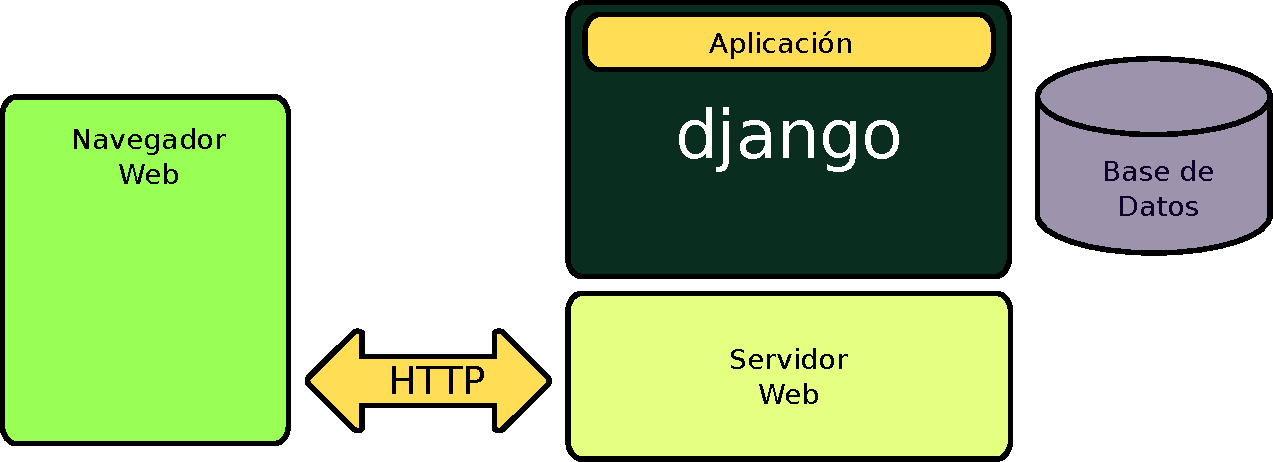
\includegraphics[scale=0.5]{fw_django.pdf}
\end{frame}

\begin{frame}
\frametitle{Framework Web - Django - Componentes}
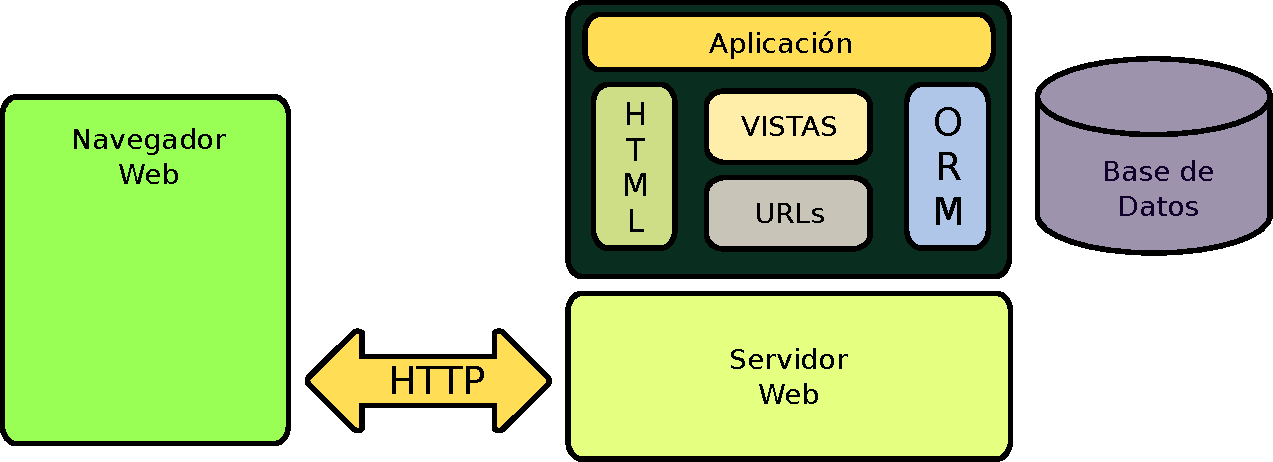
\includegraphics[scale=0.5]{fw_django_comp.pdf}
\end{frame}

\subsection{Principales Obstáculos}
\begin{frame}
    \frametitle{Carencias de los navegadores}
    \begin{itemize}
        \item{{\bf Servidor Web}\\
            Sin servidor, el navegador sólo posee la {\bf caché}}
        \item{{\bf Base de Datos} \\
            Un navegador no posee un mecanismo de almacenamiento}
        \item{{\bf Lenguaje de Programación Consistente}\\
            Cada navegador implementa a su manera {\bf JavaScript} y {\bf DOM}}
        \item{{\bf Concurrencia} \\
            Los eventos son atendidos en el bucle principal}
        \item{{\bf Conectividad con el entorno del cliente}\\
            Escritorio $\not=$ Espacio de URLs}
    \end{itemize}
\end{frame}

%\subsection{Tecnologías Existentes}
\begin{frame}
     \frametitle{Principales alternativas}
     
     
     \begin{columns}[c]
     \begin{column}{5cm}
         \itemize{
             \item {\bf Microsoft Silverlight}\\
             \item {\bf Sun JavaFX}
             \item {\bf Adobe AIR}
             \item {\bf Mozilla XUL}
         }
     \end{column}
     \begin{column}{5cm}
        
\includegraphics[scale=0.2]{microsoft_silverlight_c.jpg}\\
        
\includegraphics[scale=0.3]{javafx_logo_color_1.jpg}\\
        
\includegraphics[scale=0.16]{adobe_air_realin.png}

     \end{column}
     \end{columns}
%    \pause
%    \\
%    Esteas tecnologías se alejan de los estándares de la Web.
    % Decir que la web 2.0, desde el punto de vista tecnologico
    % tiende a integrar serivcios en una plataforma estandar abiertos (HTML, JS + libs, etc.)
    % Estos NO.
\end{frame}

\begin{frame}
    \frametitle{JavaScript}
    \par{Un lenguaje con {\it mala} reputación con:}
    \begin{itemize}
          \item Objetos
          \item Patrones Propios (Closures, Module, etc.)
          \item Muchas librerías                    
    \end{itemize}
    \vfill
    \par{
        
\includegraphics[scale=0.4]{prototype.png}\hfill
        
\includegraphics[scale=0.2]{dojo.png}\hfill  
        
\includegraphics[scale=0.4]{jquery.png}
    }
    \par{
        
\includegraphics[scale=0.2]{yui.jpg}\hfill
        
\includegraphics[scale=0.5]{DHX_logo.jpg}\hfill
        
\includegraphics[scale=0.3]{mootools.png}
    }
\end{frame}

\begin{frame}

    \frametitle{JavaScript - Según Mozilla}
    \begin{columns}[c]
         \begin{column}{5cm}
             \itemize{
                 \item Generadores e Iteradores
                 \item Varias ayudas para una mejor programación OO
                 \item Sabor Pythonico :)
             }
         \end{column}
         \begin{column}{5cm}
            
\includegraphics[scale=1.2]{mozilla.png}
            
    
         \end{column}
     \end{columns}    
\end{frame}

\begin{frame}
    \frametitle{Google Gears}
    \par{
        Plugin para los navegadores
        \hfill
        
\includegraphics[scale=0.3]{gears.png}
    }
    \begin{itemize}
        \item{\bf Local Server}
        \item{\bf Data Base}
        \item{\bf Worker Pool}
        \item{\bf Desktop}
    \end{itemize}
\end{frame}

\section{Desarrollo}
\subsection{Propuesta}
\begin{frame}
    \frametitle{Gears}
    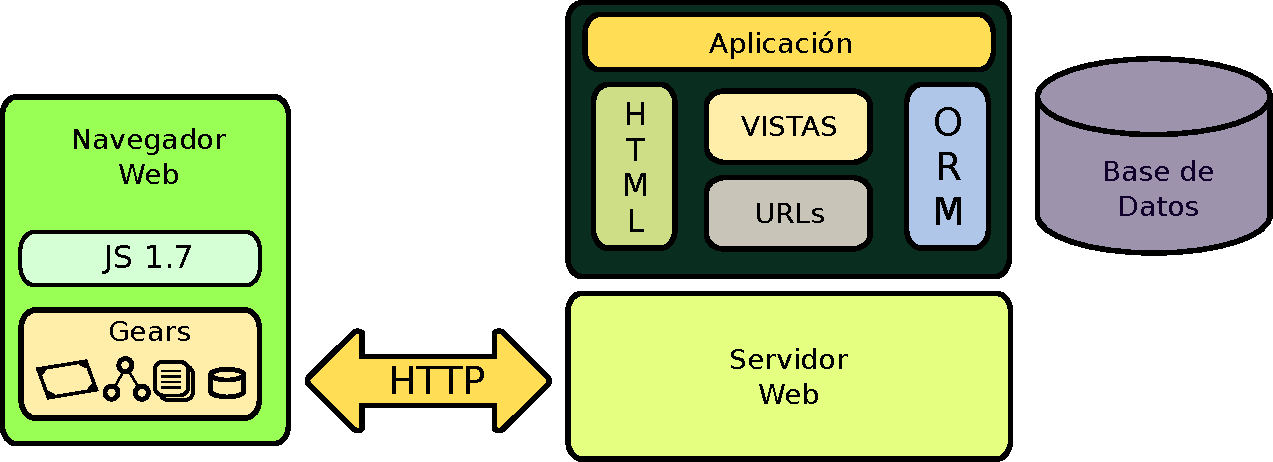
\includegraphics[scale=0.5]{fw_django_comp_gears.pdf}
\end{frame}

\begin{frame}
    \frametitle{¿Django Desconectado?}
    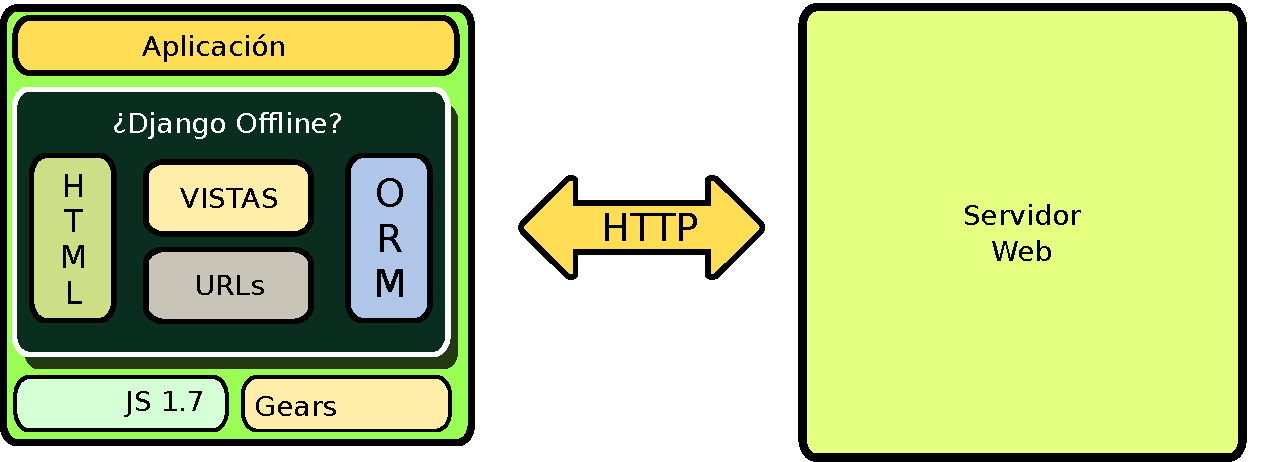
\includegraphics[scale=0.5]{fw_desconectado.pdf}
\end{frame}

\subsection{Solución}
\begin{frame}
    \frametitle{Doff y Protopy}
    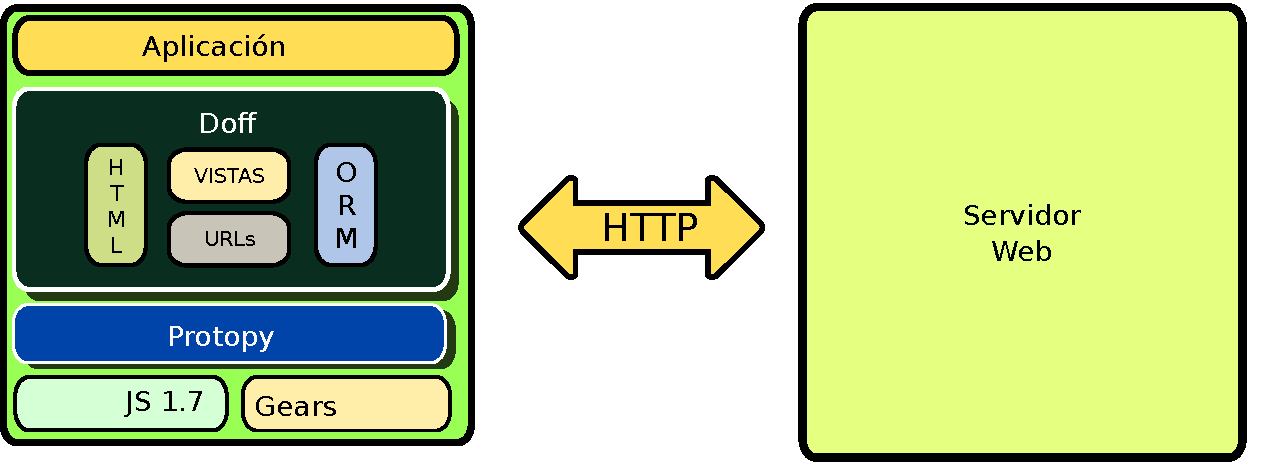
\includegraphics[scale=0.5]{fw_doff_protopy.pdf}
\end{frame}


\subsection{Librería de JavaScript}
\begin{frame}
    \frametitle{Protopy - Librería de JavaScript}
    
            {\bf Objetivos:}\par
                \begin{itemize}
                        \item{Soporte del framework desconectado}
                        \item{Interfaz Pythonica}
                        \item{Promover la reutilización de código}
                        \item{Control de la página y eventos (DOM)}
                        \item{Interfaz con las tecnologías de persistencia y ejecución offline} 
                \end{itemize}     
         
\end{frame}    
      
\begin{frame}
    \frametitle{Protopy - Componentes}
        \begin{columns}[c]
         \begin{column}{5cm}
            \begin{itemize}
                \item {\bf Módulos}
                \item {\bf Clases}
                \item {\bf DOM y Eventos}
                \item {\bf AJAX - RPC - JSON}
                \item {\bf Gears}
                \item {\bf Logging}
             \end{itemize}
         \end{column}
         \begin{column}{5cm}
            
\includegraphics[scale=0.5]{protopy.png}
         \end{column}
     \end{columns}                       
\end{frame}

\begin{frame}
    \frametitle{Protopy - Componentes}
    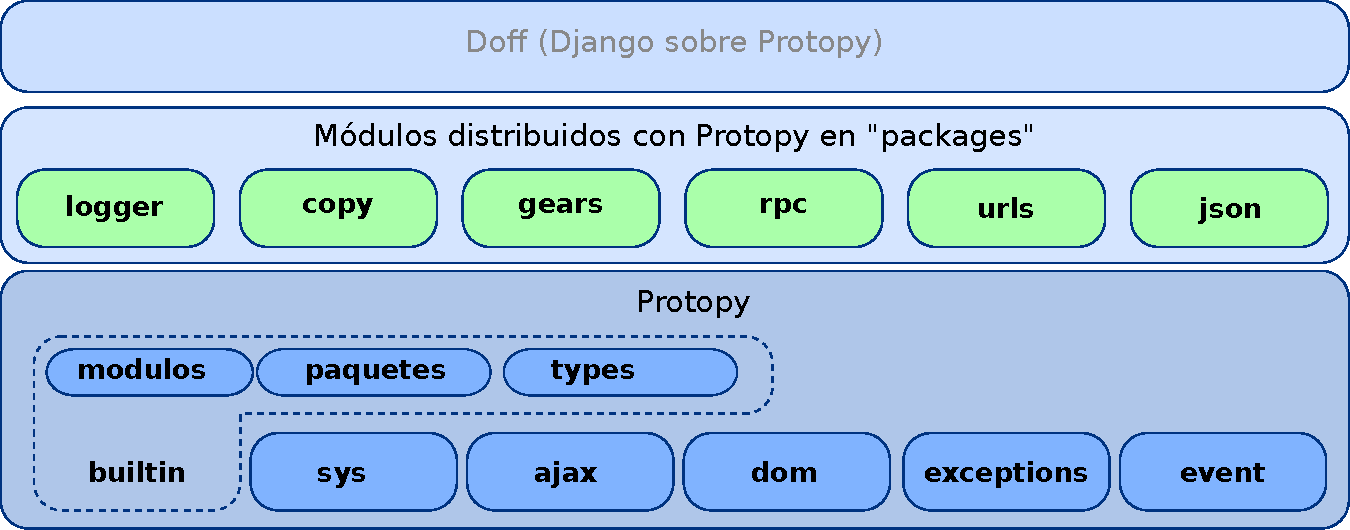
\includegraphics[scale=0.47]{esquema_protopy.pdf}
\end{frame}

\subsection{Framework Desconectados}
\begin{frame}
    \frametitle{Doff - Objetivos}
    \begin{itemize}
        \item{Facilitar el desarrollo desconectado}
        \item{Reutilización de recursos del proyecto en línea}
        \item{Emulación de HTTP}
        \item{Control de URLs e historial del navegador}
        \item{Persistencia de la aplicación, datos y {\it bootstraping}}
        \item{Sincronización}
        \end{itemize}
\end{frame}

\begin{frame}
    \frametitle{Doff - Componentes}
    \begin{itemize}
        \item {\bf API de Modelos }
        \item {\bf Templates }
        \item {\bf Formularios }
        \item {\bf URLs y Vistas }
        \item {\bf DOMAdapter y LocalHandler }
        \item {\bf Aplicaciones adicionales }
            \itemize{
                \item Sincronización, Autenticación, Sesión
            }
    \end{itemize}
\end{frame}

\begin{frame}
    \frametitle{Doff - Estructura}
    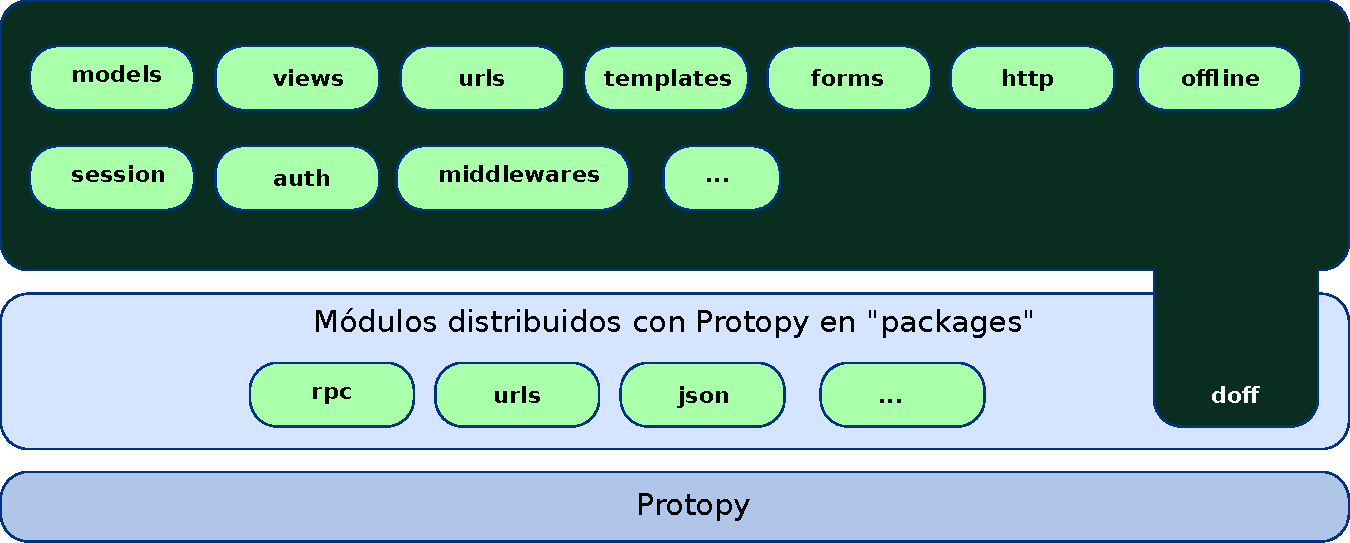
\includegraphics[scale=0.5]{esquema_doff.pdf}
\end{frame}

\begin{frame}
    \frametitle{Proyecto Desconectado}
    \begin{itemize}
        \item{Proyecto = paquete + configuración}
        \item{Escribir aplicaciones, modelos, vistas}
        \item{Escribir el mapeo de urls en vistas}
        \item{Escribir templates}
        \item{Crear el manifiesto}
    \end{itemize}
\end{frame}


\subsection{Aplicación de desconexión}
\begin{frame}
    \frametitle{Offline - Objetivos}
    \begin{itemize}
        \item{Automatización de creación de proyectos desconectados}
        \item{Servidor estático del código de Protopy y Doff}
        \item{Servidor estático del código de cada proyecto}
    \end{itemize}
\end{frame}

\begin{frame}

    \frametitle{Offline - RemoteSites}
    \par{
        \par{\bf Objetivo:}
        Definición de desconectado en el cliente. Cada sitio remoto es una {\it vista}
        del proyecto y se publica en una {\it URL}

    }
    \begin{itemize}
      \item{Conversión de modelos de Python a JS mediante {\it introspección}}
      \begin{item}Definición de acceso a datos del servidor
        \begin{itemize}
          \item {Acceso a filas ({\it managers})}
          \item {Acceso a columnas ({\it modificación de modelos})}
        \end{itemize}
      \end{item}
      \item{Publicación de plantillas}
    \end{itemize}

\end{frame}

\begin{frame}

    \frametitle{Offline - RemoteSites estructura}
    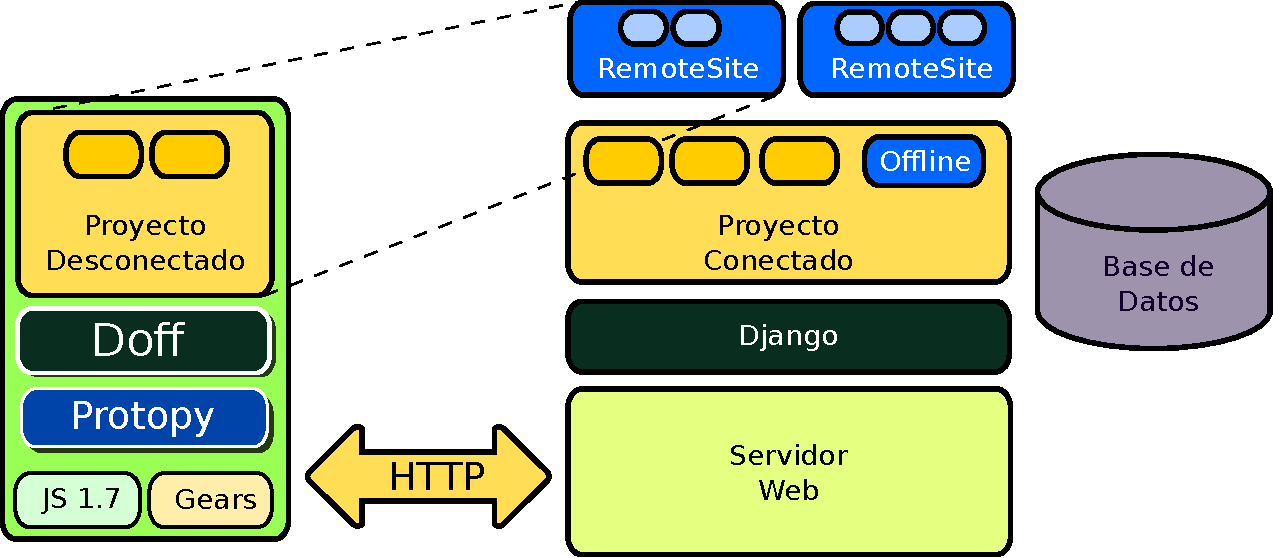
\includegraphics[scale=0.5]{remote_sites.pdf}
    
\end{frame}

\begin{frame}
    \frametitle{Offline - Aplicación del cliente}
    \begin{itemize}
      \item{Soporte en el cliente para la instalación de un RemoteSite}
      \item{Modelos base para los modelos que se desconecten de {\bf offline}}
      \item{Managers remotos y managers que trabajan con la consistencia}
      \item{Manejador de Sincronización}
      \item{Agrega elementos al contexto de renderización para identificar
            estado}
    \end{itemize}
\end{frame}

\section{Sincronización}
\begin{frame}
    \frametitle{Sincronización - Esquema}
    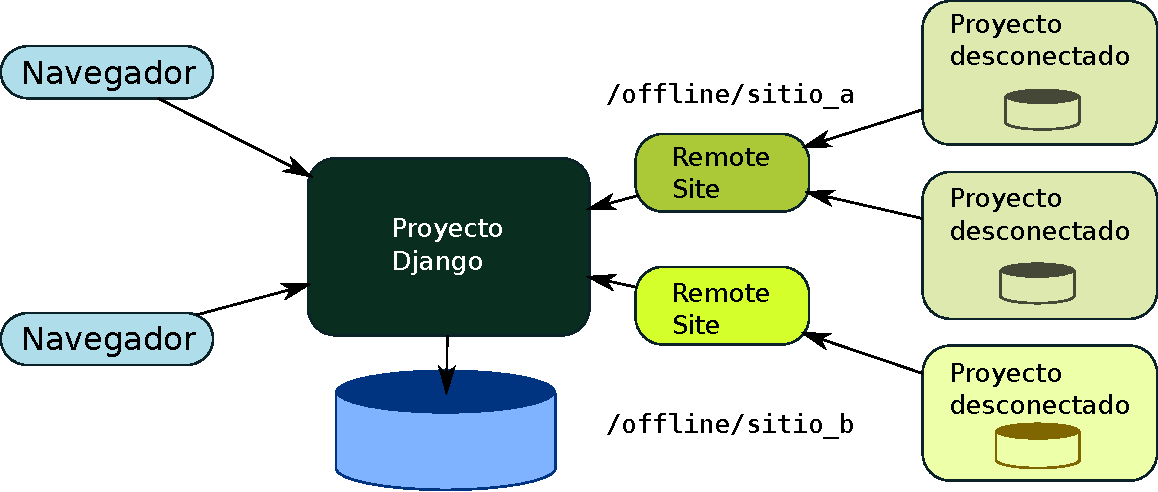
\includegraphics[scale=0.5]{esquema_distribuido.pdf}
\end{frame}

\subsection{Objetivo}
\begin{frame}
    \frametitle{Sincronización - Objetivo}
    \par {
    	Que las entidades definidas en el servidor se repliquen en el cliente, y
    	que las creadas y modificadas en el cliente se transfieran al servidor
    }
    \par
    \pause
    \begin{itemize}
        \item{Integridad de la sincronización}
		\item{Transporte de datos}
		\begin{item}
          \par{Detección de cambios en instancias en el servidor}
		  \begin{itemize}
            \item{SyncData aprovechando el ContentType framework}
            \item{Señales}
          \end{itemize}
		\end{item}
        \begin{item}
          Detección de cambios en el cliente
          \begin{itemize}
                \item{server\_pk}
                \item{active}
                \item{sync\_log}
                \item{status}
          \end{itemize}
        \end{item}
    \end{itemize}
\end{frame}

\subsection{Primitivas}
\begin{frame}
    \frametitle{Sincronización - Primitivas}
    	\begin{itemize}
            \item{\bf PULL - Cliente/Servidor}
            	\begin{itemize}
                	\item{data}
                	\item{sync\_log}
          		\end{itemize}
            \item{\bf PUSH - Cliente/Servidor}
            	\begin{itemize}
                	\item{need\_pull}
                	\item{chunked}
                	\item{deleted, modified, created}
                	\item{sync\_log/s}
          		\end{itemize}
            \item{\bf PURGE - Cliente}
            	\begin{itemize}
                	\item{active}
                	\item{status}
                \end{itemize}
            \item{\bf UPDATE - Cliente} 
        \end{itemize}
\end{frame}

\begin{frame}
    \frametitle{Ciclo de vida de una entidad}
    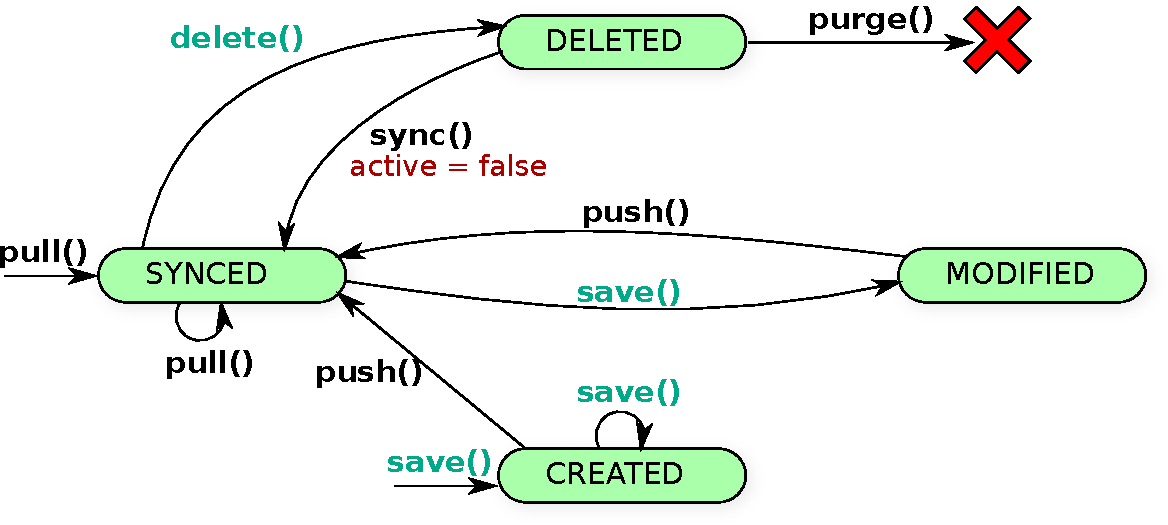
\includegraphics[scale=0.55]{esquema_sync_client.pdf}
\end{frame}

\subsection{Conflictos}
\begin{frame}
    \frametitle{Sincronización - Conflictos}
    \par{
    Se provee un mecanismo básico de resolución de conflictos que 
    puede ser extendido en función del dominio de la aplicación
    }
    \begin{itemize}
      	\item{Middleware de sincronización}
        \item{Los conflictos se resuelven en el cliente}
        \begin{item}
        \par{
        	Detección de conflictos en base a atributos agregados por
        	{\bf offline}
        }
        \begin{itemize}
          \item{Unicidad en la base de datos}
          \item{Modificación local vs Modificación remota}
          \item{Eliminación local vs Modificación remota}
          \item{Modificación local vs Eliminación remota}
        \end{itemize}
        \end{item}        
    \end{itemize}
\end{frame}

\section{Conclusiones}
\subsection{Objetivos Cumplidos}
\begin{frame}
    \frametitle{Conclusiones}
    \begin{itemize}
        \item {\bf Extender un framework $\surd$}
        \item {\bf Persistencia del modelo de datos en el cliente $\surd$}
        \item {\bf Acciones disponibles en modo desconectado $\surd$}
        \item {\bf Primitivas de sincronización $\surd$}
        \item {\bf Desarrollo de software libre $\surd$}

    \end{itemize}
\end{frame}

\subsection{Líneas Futuras}
\begin{frame}
    \frametitle{Líneas Futuras}
    \begin{itemize}
        \item {\bf Conversión de Código Python en JavaScript}
        \item {\bf Sitio de Administración}
        \item {\bf Workers con Soporte para JavaScript 1.7}
        \item {\bf Compatibilidad con ES5 y HTML5}
        \item {\bf Optimizaciones en Base a Permanencia de Estado}
        \item {\bf Implementación de Storage o Almacenamiento en el Cliente}
        \item {\bf Compilación de JavaScript}
        \item {\bf Manejo de Migraciones de Esquema}
    \end{itemize}
\end{frame}

\subsection{Herramientas Open Source}
\begin{frame}
    \frametitle{Miscelánea}
    \begin{itemize}
        \item {\bf Firefox} Plataforma
        \item {\bf Firebug} Depuración
        \item {\bf Django} Framework Web
        \item {\bf Python} Lenguaje Server Side, Scripting, Sphinx Hacking, etc.
        \item {\bf Mercurial} Control de versiones
        \item {\bf Sphinx} Para crear la documentación, \LaTeX{} y HTML
        \item {\bf \LaTeX{} - beamer} Para crear {\it esta} presentación
    \end{itemize}
\end{frame}

\begin{frame}
    \begin{center}
        \vfill
        
\includegraphics[scale=0.3]{protopy.png}\par
        {\LARGE\bf http://code.google.com/p/protopy}
        \vfill
    \end{center}    
\end{frame}

\begin{frame}
    \vfill
    \begin{center}
        {\Huge\bf ¡¡¡Muchas Gracias!!!}
    \end{center}
    \vfill
\end{frame}
\end{document}
